\section{Project Status}
\label{sec:project-status}

\subsection{Modeling Time Drift}
\label{sec:modeling-time-drift}
In previous implementations, we modeled clocks generating an event for each clock tick. Modeling drift reduced to slightly changing the rate of clock events generation for each node.
The actual implementation we don't have an event for each clock tick, and drift has been modeled using the Ptolemy support for multiform time. Figure \ref{fig:time} shows clocks drift for two nodes in our model.

\begin{figure}
  \centering
  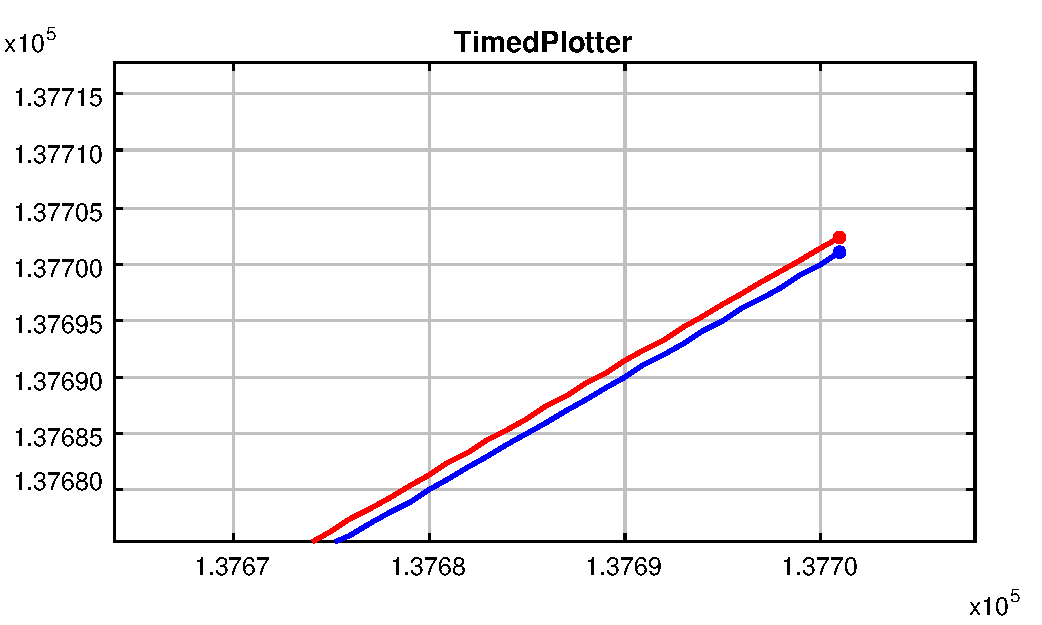
\includegraphics[width=\textwidth]{figures/time-drift.pdf}
  \caption{Time drift modeling in Ptolemy using Multiform time}
  \label{fig:time}
\end{figure}

\subsection{Modeling the IEEE 802.15.4e state machine}
\label{sec:modeling-state-machine}

We modeled the IEEE 802.15.4e finite state machine using Ptolemy modal modes. The result is the hierarchical FSM shown in figure \ref{fig:fsm}. Figure \ref{fig:tx} shows the refinement of the TX state of the high level FSM. All other states of the high level FSM, RX, SLEEP and SYNC, are similarly refined.

\begin{figure}
  \centering
  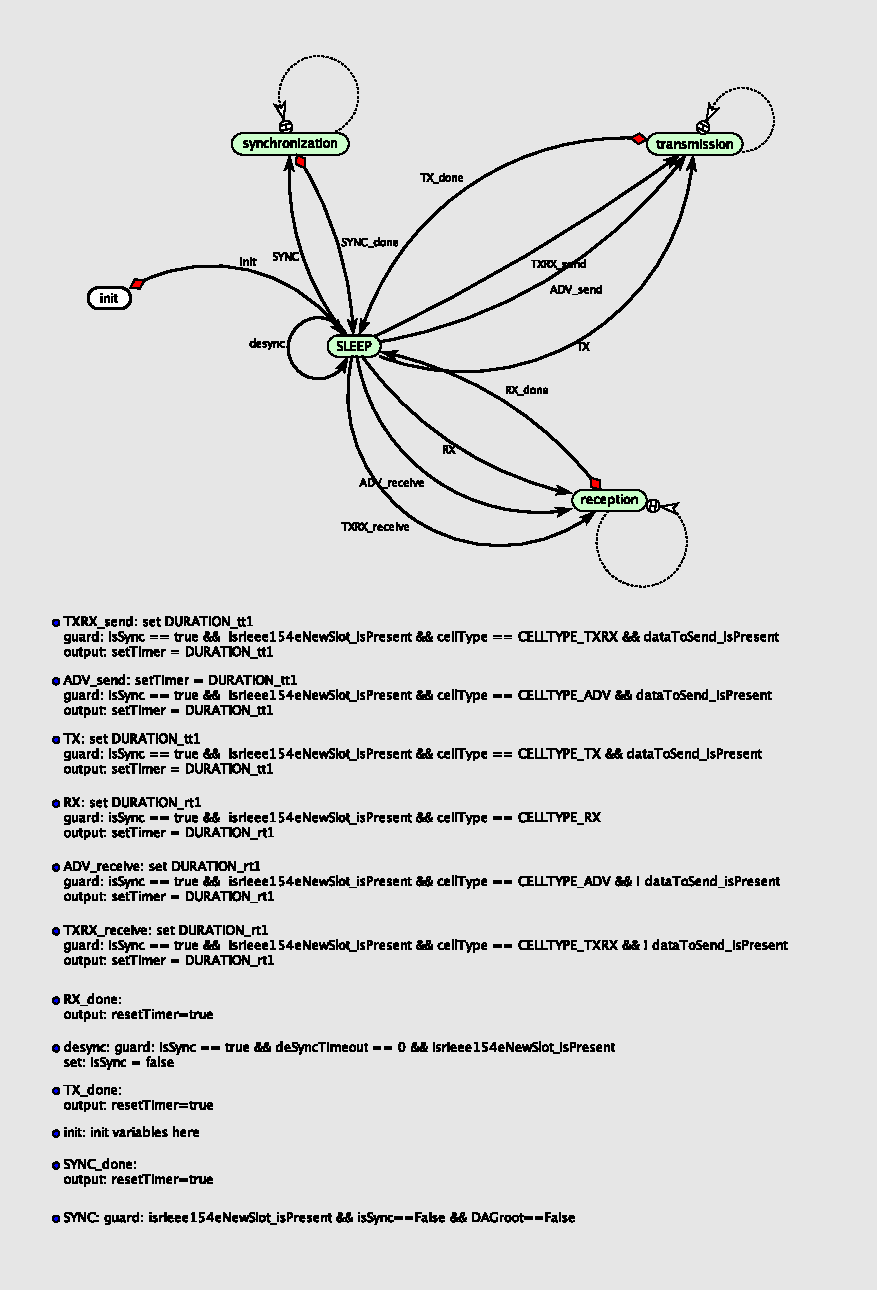
\includegraphics[width=\textwidth]{figures/FSM.pdf}
  \caption{High level FSM of the IEEE 802.15.4e protocol standard}
  \label{fig:fsm}
\end{figure}

\begin{figure}
  \centering
  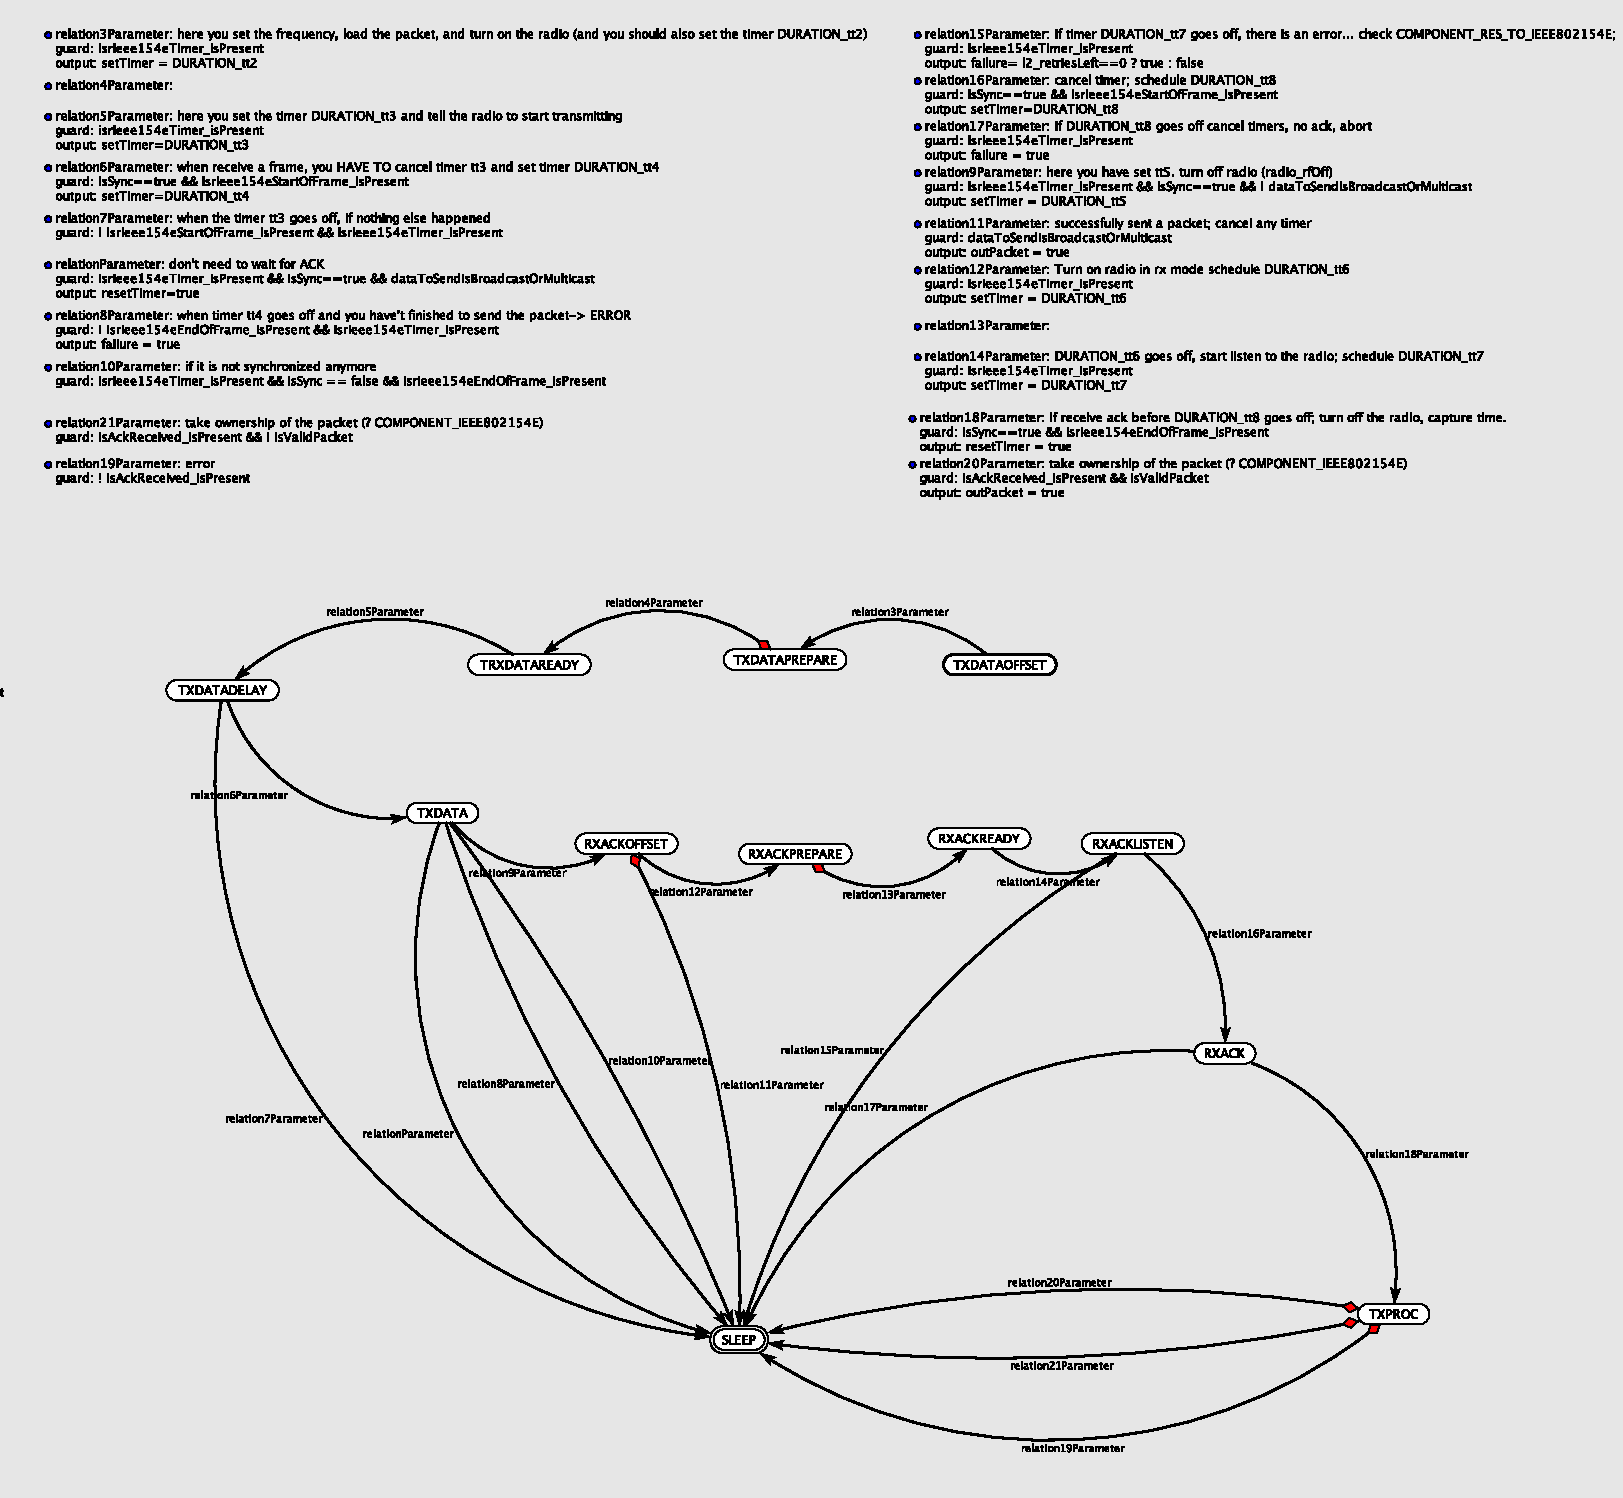
\includegraphics[width=\textwidth]{figures/TransmissionFSM.pdf}
  \caption{Transmission state refinement}
  \label{fig:tx}
\end{figure}

\subsection{Modeling the Physical Layer}
\label{sec:modeling-physical-layer}
Physical layer is modeled as a discrete event model. The physical layer is used to communicate with the MAC layer information such us the beginning and the end of the reception of a packet. Figure \ref{fig:node} shows the actual structure of a node model (a DE model), including the relation between the physical and the MAC layer.

\begin{figure}
  \centering
  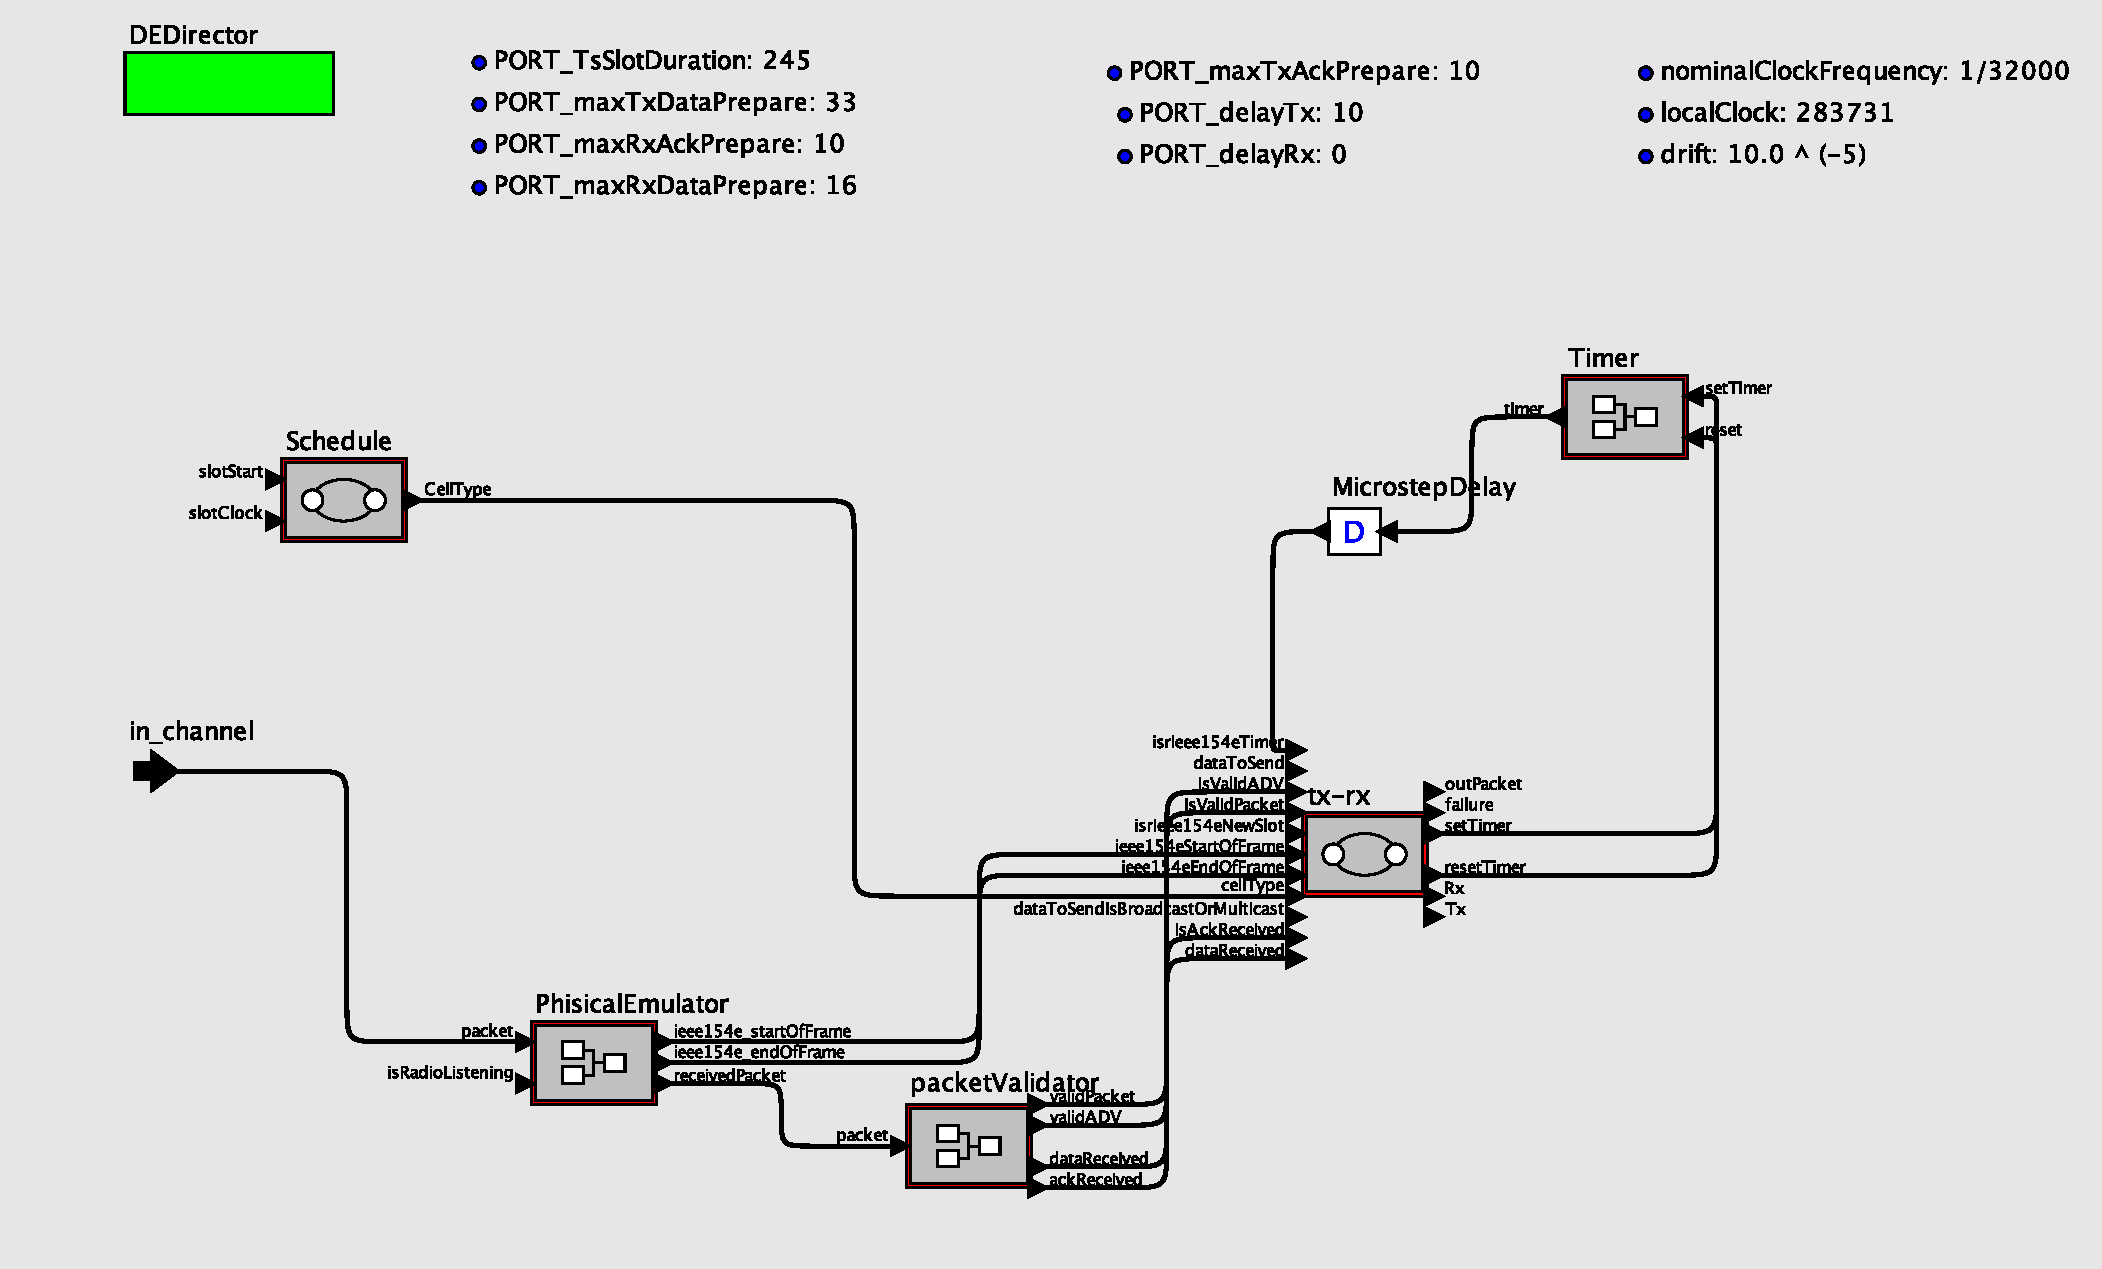
\includegraphics[width=\textwidth]{figures/WirelessNode.pdf}
  \caption{Interaction between different actors composing a node}
  \label{fig:node}
\end{figure}


\subsection{Modeling the scheduler}
\label{sec:modeling-scheduler}
In our model, the scheduler is represented as a FSM. At this point, we don't support a dynamic scheduler. We think this is not a limitation, also because the actual OpenWSN firmware uses an hardcoded scheduler. In particular, our implementation of the scheduler follows the OpenWSN implementation. Figure \ref{fig:scheduler} shows our implementation of the scheduler. Unconnected states represent other available slot types, not used in the OpenWSN implementation.

\begin{figure}
  \centering
  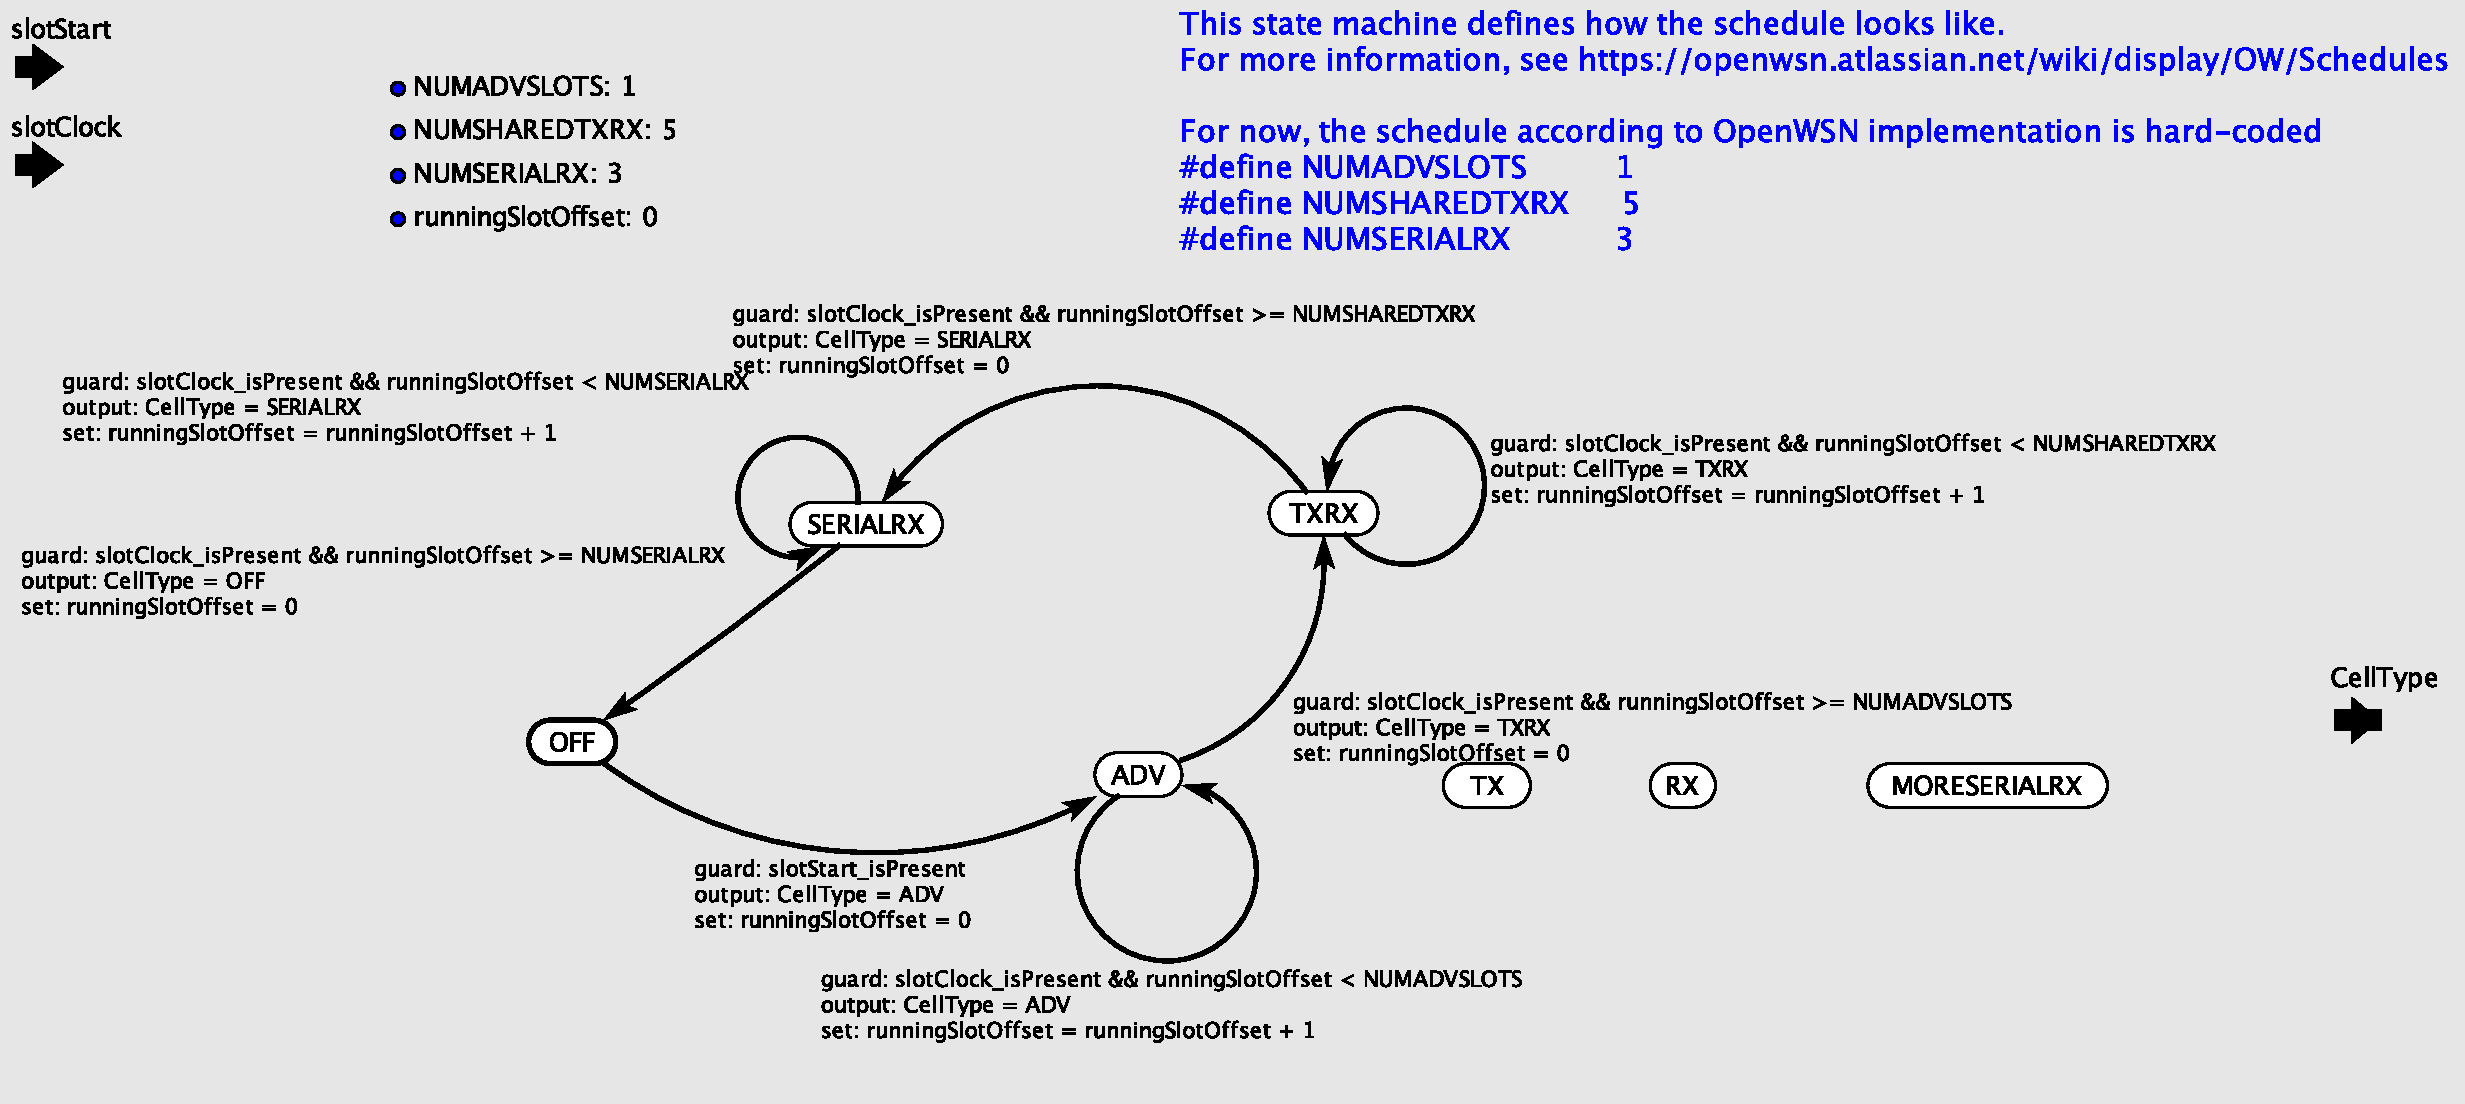
\includegraphics[width=\textwidth]{figures/Scheduler.pdf}
  \caption{Scheduler FSM}
  \label{fig:scheduler}
\end{figure}

%%% Local Variables: 
%%% mode: latex
%%% TeX-master: "report"
%%% End: 
